%% PAQUETES
\usepackage[utf8]{inputenx}
\usepackage[spanish]{babel}
\usepackage{amsmath}
\usepackage{amsthm}
\usepackage{amssymb}
\usepackage{amsfonts}   
\usepackage{pifont}     % Para tickYes y tickNo
\usepackage{graphicx}
\usepackage{epsfig}
\usepackage{pdflscape}
\usepackage{enumerate}
\usepackage{color}
\usepackage{beamerfoils}
\usepackage{beamerprosper}
\usepackage{xspace}
\usepackage{booktabs}
\usepackage{multicol}
\usepackage{multirow}
\usepackage{tikz}
\usepackage{pgflibraryshapes}
\usepackage{wasysym}
\usepackage{float}
\usepackage{listings}

%% CONFIGURACIÓN DE TIKZ
% Librerías cargadas
\usetikzlibrary{arrows}
%\usetikzlibrary{calc,fadings,decorations.pathreplacing,arrows,intersections,
%    decorations.markings,external,shapes}

% Configuración de Tikz y Pgfplot
\tikzset{%
    >=stealth, % option for nice arrows
    inner sep=0pt,%
    outer sep=3pt,%
    mark coordinate/.style={inner sep=0pt,outer
    sep=0pt,minimum size=3pt,
    fill=black,circle}%
    }

% Librerías de tiKz
    %\usetikzlibrary{}

    % Define block styles
\tikzstyle{io} = [trapezium,trapezium left angle=70,trapezium right angle=-70,
  minimum height=0.9cm, draw, fill=blue!20, text width=4.5em, 
  text badly centered, node distance=2cm, inner sep=0pt]
\tikzstyle{decision} = [diamond, draw, fill=blue!20, text width=5.5em, 
  text badly centered, node distance=2cm, inner sep=0pt]
\tikzstyle{block} = [rectangle, draw, fill=blue!20, text width=5em, 
  text centered, rounded corners, minimum height=4em]
\tikzstyle{line} = [draw, -latex']
\tikzstyle{cloud} = [draw, ellipse,fill=red!20, node distance=2cm, 
    minimum height=2em]


%% TEMAS BASE
\usetheme{Boadilla}
\setbeamertemplate{headline}{
\begin{beamercolorbox}{section in head/foot}
\vskip2pt\insertnavigation{\paperwidth}\vskip2pt
\end{beamercolorbox}

\includegraphics[width=\paperwidth]{images/ucm_logo}}

\usecolortheme{lily}

\useinnertheme{circles}

\definecolor{ZurichBlue}{rgb}{.255,.41,.884}
\setbeamercolor{alerted text}{fg=ZurichBlue}
\definecolor{Comentario}{rgb}{0.0,0.5,0.0}

%% CONFIGURACIÓN GEENERAL DE HIPERVÍNCULOS
\hypersetup{%
    baseurl={roberto.antolin@mat.ucm.es},
    pdftitle={Filtro LiDAR. Ejemplo práctico: GRASS},%
    pdfauthor={Roberto Antol\'{i}n S\'anchez},%
    pdfcreator={Roberto Antol\'{i}n S\'anchez},%
    pdfproducer=PDFLaTeX,%
    pdfsubject={LiDAR GRASS data filtering},%
    pdfkeywords={filtros, splines, LiDAR, GRASS}%
  }

\mode<presentation>{\hypersetup{pdfpagemode=FullScreen}}

%% COMANDOS
% Tipos de datos
\newcommand{\file}[1]{\path{#1}\xspace} %Referencias a ficheros
\newcommand{\extr}[1]{\emph{#1}\xspace} %Palabras extranjeras
\mode<article>{\newcommand{\soft}[1]{\textsf{#1}\xspace} }%Referencias a software
\mode<presentation>{\newcommand{\soft}[1]{\textrm{#1}\xspace} }%Referencias a software
\newcommand{\sigl}[1]{\textsc{#1}\xspace} %Siglas
\newcommand{\nota}[1]{\textcolor{nota}{�#1?}\xspace}
\newcommand{\frametitlee}[1]{\mode<presentation| handout| article:0>{\frametitle{#1}}}
\newcommand{\figuree}[2]{
  \mode<article>{
    \begin{figure}[H]
    \centering
    }
    #1
    \mode<article>{
    \caption{#2}
    \end{figure}
  }
}

% Atajos
\newcommand{\inet}{\extr{Internet}}
\newcommand{\html}{\sigl{html}}
\newcommand{\web}{\extr{web}}
\newcommand{\software}{\extr{software}}
\newcommand{\hardware}{\extr{hardware}}
\newcommand{\tickNo}{\color{red}\ding{55}}
\newcommand{\tickYes}{\color{green!50!black}\checkmark}

%% PREFERENCIAS PARA LISTINGS (código)
\lstdefinestyle{mio}{
  basicstyle=\ttfamily\scriptsize,%
  keywordstyle=\bfseries\color{ZurichBlue},%
  commentstyle=shape\color{green},%
  stringstyle=\color{red!50!black},
}

\lstdefinestyle{latex}
{
language={[latex]tex},
keywordstyle=\color{resalta!50!black},
commentstyle=\color{fondoO!50!green}\itshape
}

\lstdefinestyle{shell}{
  language=sh,
  basicstyle=\ttfamily\scriptsize,%
  morekeywords={lasinfo,lasdiff,lasmerge,las2txt,txt2las,las2ogr,laszip,
    lasview, lasboundary, lasgrid, lasduplicate, lasoverlap,
    las2dem, las2las, lastile, lasground, lasheight, lasclassify},
  keywordstyle=\bfseries\color{ZurichBlue},
  commentstyle=\color{green!35!black}%
}

\lstdefinestyle{grass}{                                                                     
  language=sh,
  basicstyle=\ttfamily\scriptsize,%
  morekeywords={v.lidar.edgedetection,v.lidar.growing,
  v.lidar.correction,v.surf.bspline,v.outlier},
  keywordstyle=\bfseries\color{ZurichBlue},classoffset=1,
  commentstyle=shape\color{green!75!black},%
  morekeywords={GRASS6 (stuttgart):, >}
  keywordstyle=\color{green!50!black}, classoffset=0
}

%
\lstdefinestyle{matlab}{
  basicstyle=\scriptsize\ttfamily,
  breaklines=true,
  commentstyle=\color{Comentario},
  keywordstyle=\bfseries\color{blue},
  language=Matlab,
  %xleftmargin=\parindent,
  identifierstyle=\bfseries
}

\lstset{style=mio,
   tabsize=4,%
   inputencoding=utf8,%latin1,%
   extendedchars=true,%
   breaklines=true,%
   showstringspaces=false,
   backgroundcolor=\color{gray!20!white}
   }

%% DATOS DEL DOCUMENTO
\title[FOSS para trabajar con LiDAR]
    {Filtro LiDAR. Ejemplo práctico: GRASS}

\author[R. Antolín]
    {Roberto Antolín Sánchez}

\institute[UCM]{
        Prof. Titular Interino
	Sec. Dptal. Astronomía y Geodesia\\
        Facultad de CC. Matemáticas (UCM)\\
	Plaza de Ciencias, 3\\
	Madrid -- 28040\\
	\texttt{roberto.antolin@mat.ucm.es}\\
}

%% FECHA DE LA PRESENTACIÓN
\date[06-05-2013]{6 de Mayo de 2013}

\AtBeginSection[]
{
  \begin{frame}[shrink=20]
    \frametitle{Table of Contents}
    \tableofcontents[currentsection,hidesubsections]
  \end{frame}
}

\begin{document}
%\includeonlyframes{cc}
%intro3,intro4,funciona,ventajas1,ventajas2,ventajas3
%desventajas,miktex,miktex2,editores,otrasherr
%%================================================================== Logo On/Off
\LogoOff

%==================================================================FRONT PAGE AND TOC
% For article only
\mode<presentation:0>{\thispagestyle{empty}\maketitle}

% For presentation only
\mode<presentation| article:0| handout:0>{
    \begin{frame}<article:0>[label=portada]
    \titlepage
    \end{frame}%Fin del frame
}

% For handout only
\mode<handout>{
  \begin{frame}[label=portada]
    \maketitle
  \end{frame}
}

%% TABLE OF CONTENTS
\begin{frame}[label=toc]
    \mode<article:0>{\frametitle{Contents}}
    \mode<presentation>{\small}
    \tableofcontents%[hidesubsections]
\end{frame}

%%%==================================================================S INTRODUCTION
\section{\textquestiondown Qué es el LiDAR aéreo?}
%%%==================================================================Sb
%\subsection{Principios}
%%%==================================================================F 
%\begin{frame}
%    \frametitle{Principios del LiDAR aéreo}
%    \begin{enumerate}
%        \item El LiDAR aéreo (Airborne Laser Scanner, \alert<1>{ALS}) es la combinación de:
%	\uncover<1->{
%	\begin{itemize}
%	 \item \alert<1,2>{Escaner Laser}
%	 \item \alert<1,3>{GPS}, que nos da la posición del sensor.
%	 \item \alert<1,3>{IMU}, que nos da nuestra orientación del avión.
%	\end{itemize}
%	}
%	\uncover<2->{
%	\item La posición con respecto al sensor de un punto en tierra se determina por:
%	\begin{itemize}
%	 \item El \alert<2>{tiempo} que tarda cada impulso desde que es emitido hasta que es recibido.
%	 \item El \alert<2>{ángulo} medido desde el nadir en el cual ha sido emitido el rayo.
%	\end{itemize}
%	}
%	\uncover<3>{\item  La posición relativa combinada con la posición global (\alert<3>{GPS}) y la orientación (\alert<3>{IMU}) nos permiten calcular las coordenadas (X,Y,Z) en el punto medido en tierra en un sistema de posicionamiento global (WGS84)}
%    \end{enumerate}
%\end{frame}
%%%==================================================================Sb
%\subsection{Características}
%%%==================================================================F
%\begin{frame}[label=lidar_charact]
%    \frametitle{Características del ALS}
%    \begin{enumerate}[<+->]
%    	\item \alert<1>{Alta precisión} tanto en la componente planimétrica como en la altrimétrica
%    	\item \alert<2>{Alta resolución} debido a la frecuencia de medición.
%    	\item \alert<3>{Monoscópica} y casi \alert{nadiral} $\Rightarrow$ permite observar el terreno incluso en zonas de gran vegetación
%    \end{enumerate}
%\end{frame}
%%==================================================================Sb
\subsection{Primer y último impulso}
%%==================================================================F 
\mode<beamer>{
  \pgfdeclareimage[height=40mm]{roof}{images/roof}
  \pgfdeclareimage[height=40mm]{tree}{images/tree}
}
\mode<beamer:0>{
  \pgfdeclareimage[height=40mm]{roofg}{images/roof_grey}
  \pgfdeclareimage[height=40mm]{treeg}{images/tree_grey}
}
\begin{frame}[label=firstlast1]
    \frametitle{Primer y último impulso}
    \begin{enumerate}[<+->]
        \item Debido a la divergencia del láser, pueden recibirse \alert<1>{más de un eco} para el mismo rayo.
	\item Los sensores actuales son capaces de medir al menos dos retornos: \alert<2>{primero} y \alert<2>{último}
	\item Normalmente se producen por: \alert<3->{bordes} de edificios \uncover<4->{o \alert<4>{vegetación}}
    \end{enumerate}
    \begin{center}
   	\begin{tikzpicture}
	\mode<beamer>{
    	  \uncover<3->{\pgftext[bottom,left,at={\pgfpointxy{-2}{0}}]{\pgfuseimage{roof}}}
    	  \uncover<4>{\pgftext[bottom,left,at={\pgfpointxy{2}{0}}]{\pgfuseimage{tree}}}
	}
	\mode<beamer:0>{
    	  \pgftext[bottom,left,at={\pgfpointxy{-2}{0}}]{\pgfuseimage{roofg}}
    	  \pgftext[bottom,left,at={\pgfpointxy{2}{0}}]{\pgfuseimage{treeg}}
	}
	\end{tikzpicture}
    \end{center}
\end{frame}
%%==================================================================F 
\begin{frame}
    \frametitle{\textquestiondown Para qué sirve?}
    \begin{enumerate}[<+->]
     \item Una diferencia considerable entre el primer y último impulso puede ser una pista para detectar vegetación y otros objetos: edificios, puentes, tendidos eléctricos...
     \item Los últimos impulsos tienen más probabilidad de ser terreno.
     \item Mediante una simple interpolación:
     	\begin{itemize}
     	   \item Primer impulso: creación de Modelo Digital de Superficie (\alert<4>{DSM})
     	   \item \'Ultimo impulso: ``creación'' de Modelo Digital del Terreno (\alert<5>{DTM})
     	\end{itemize}
     \item Hay pocas posibilidades de, sin hacer ningún análisis, distinguir entre un punto \alert<6>{objeto} y uno \alert<6>{terreno}.
    \end{enumerate}
\end{frame}
%%==================================================================S
\section{Filtros ALS}
%%==================================================================Sb
\subsection{Definición}
%%==================================================================F
\begin{frame}[label=filter_def]
    \frametitle{Filtros ALS}
    \onslide<1->\begin{beamerboxesrounded}[shadow=true]{Definición: \emph{Nube de puntos LiDAR}}
     Es un conjunto de puntos tridimensionales con un atributo asociado: $V = \left\lbrace v=\left(x,a\right) | x \in \mathbb{R}^3, a \in \mathbb{N} \right\rbrace$
    \end{beamerboxesrounded}

    \onslide<2->{Clasificación la nube de puntos como:
    \begin{itemize}
 	\item 1, si el punto pertenece a un \alert<2>{objeto}
 	\item<3-> 0, si el punto pertenece al \alert<3>{terreno}
    \end{itemize}}

    \onslide<4>\begin{beamerboxesrounded}[shadow=true]{Definición: \emph{Filtrar}}
     Consiste en \alert<4>{eliminar} los puntos de $V$ con atributo igual 1 (objeto) y dejar los clasificados como 0 (terreno).
    \end{beamerboxesrounded}
\end{frame}
%%==================================================================Sb
\subsection{Tipos de filtros/clasificaciones}
%%==================================================================F
\begin{frame}
    \frametitle{Tipos de clasificaciones}
    \begin{itemize}
        \item Morfológicos
        \item Densificación progresiva
        \item Segmentación y \emph{clustering}
        \item Basado en superficies
        \item Estudio de pendientes (splines)
    \end{itemize}
\end{frame}
%%==================================================================Sb
\section{Comparación de filtros}
%%==================================================================F
\begin{frame}
  \frametitle{Comparación de filtros}
    \begin{itemize}
      \item Estudio del rendimiento de los 8 filtros distintos 
      \item Auspiciado por el \emph{International Society of Photogrammetry and
        Remote Sensing} (\alert{ISPRS})
      \item Estudio cualitativo y cuantitativo
    \end{itemize}
\end{frame}
%%==================================================================F
\begin{frame}
  \frametitle{Resultados}
  \begin{enumerate}
    \item Todos los filtros funcionan correctamente con escenarios poco exigentes
      \begin{itemize}
        \item Poca o nula pendiente, y extensas zonas de terreno
        \item Pequeños edificios
        \item Vegetación dispersa
      \end{itemize}
    \item Mayores problemas en zonas con:
      \begin{itemize}
        \item Edificios voluminosos con escasa extensión de terreno
        \item Parches de terreno a diferentes alturas o con alturas variables
      \end{itemize}
    \item<2-> Mejores prestaciones: \alert<2>{densificación progresiva} y los basados
      en la \alert<2>{determinación de superficies}
    \item<3-> Los más desarrollados: \alert<3>{segmentación y clustering}
    \item<4-> \alert<4>{Combinación} de varios algoritmos e \emph{inputs} distintos
  \end{enumerate}
\end{frame}
%%==================================================================F
\begin{frame}
  \frametitle{Automatización Vs Manual}
  \begin{enumerate}
    \item Comparados con la fotogrametría, los filtros son procesos \alert{automáticos}
    \item Todavía no se ha encontrado un filtro completamente automático y
      \alert{universal}
    \item \alert{Necesaria} una revisión manual
      \begin{itemize}
        \item Zonas urbanas 
        \item \alert{Innecesaria en zonas rurales}
        \item Puentes y pasos elevados
        \item Algoritmos basados en relaciones geométricas de puntos vecinos
        \item El terreno no puede ser identificado por escasez de puntos
        %\item El trabajo depende de las características de la superficie
      \end{itemize}
    \item Fuentes de datos adicionales pueden disminuir la revisión
      \begin{itemize}
        \item Delimitación de edificios
        \item Contexto de terreno local
        \item Información radiométrica: \alert{externa} o la \alert{devuelta por
          el láser}
      \end{itemize}
  \end{enumerate}
\end{frame}
%%==================================================================F
\begin{frame}
  \frametitle{Densidad puntual}
  \begin{itemize}
    \item La influencia de la densidad depende fuertemente de la topografía
    \item Se necesita una densidad mínima para asegurar cierta penetración en
      zonas vegetales
    \item En zonas complejas es además importante para asegurar la
      representación de calidad de los detalles del escenario
    \item Incluso con alta densidad, los filtros presentan problemas de
      clasificación
    \item Según disminuye la densidad los resultados empobrece rápidamente
  \end{itemize}
\end{frame}
%%==================================================================Sc
\section{Generación de Modelos Digitales del Terreno}
%%==================================================================F
\begin{frame}
  \frametitle{Modelos Digitales del Terreno (DTM)}
  \begin{beamerboxesrounded}[shadow=true]{Definición}
    Teóricamente sería una representación continua, $f$, del terreno en un
    cierto área local. Dadas las coordenadas planimétricas de un punto,
    $\mathbf{p}=(x,y)$, y su valor altimétrico asociado, $z$, la representación 2.5D del terreno, sería: $z=f(x,y)$
  \end{beamerboxesrounded}

  \begin{enumerate}
    \item  a
      \begin{itemize}
        \item  a
      \end{itemize}
  \end{enumerate}
\end{frame}
%%==================================================================F
\begin{frame}
  \frametitle{A}
  \begin{enumerate}
    \item A
      \begin{itemize}
        \item  A
      \end{itemize}
  \end{enumerate}
\end{frame}
%%==================================================================Sc
\subsection{Reducción de los datos}
%%==================================================================F
\begin{frame}
  \frametitle{Densidad puntual}
  \begin{enumerate}
    \item \alert{Todavía} es importante una reducción de la densidad
      puntual\alert{!}
    \item Escaneo: $100$ KHz $\Rightarrow$ \alert{$\approx$ 10
      pts/$\mathrm{m}^2$} $\Rightarrow$ Alta resolución en el DTM
    \item Problemas de almacenamiento y procesado
    \item Necesaria una reducción de la densidad
    \item Métodos
      \begin{itemize}
        \item Cambio de la estructura del DTM
        \item Sin cambio de la estructura del DTM
      \end{itemize}
  \end{enumerate}
\end{frame}
%%==================================================================F
\begin{frame}
  \frametitle{Remuestreo}
  \begin{enumerate}
    \item Métodos estándar en el procesado de imágenes digitales
    \item Menor resolución con celdas más grandes
    \item El valor del píxel nuevo se deriva de las celdas originales
    \item<2-> \alert<2>{Ventajas}
      \begin{itemize}
        \item Aplicable también para mallas
        \item Muy rápido y mantiene la estructura
      \end{itemize}
    \item<3-> \alert<3->{Desventajas}
      \begin{itemize}
        \item No son adaptativos: presentan problemas con diferencia de alturas
         \begin{itemize}
           \item<4-> Raster adaptativos locales\only<5>{: \alert{poco usados}}
         \end{itemize}
      \end{itemize}
  \end{enumerate}
\end{frame}
%%==================================================================F
\begin{frame}
  \frametitle{TIN's}
  \begin{enumerate}
    \item \alert<1-3>{Purga de puntos}
      \begin{itemize}
        \item<2-> Considera el TIN completo 
        \item<3-> elimina puntos paso a paso
      \end{itemize}
    \item \alert<4-5>{Aproximación por subdivisión}
      \begin{itemize}
        \item<4-> Empieza con un TIN aproximado
        \item<5-> Utiliza algoritmos \alert<5>{divide y vencerás} hasta alcanzar cierto
          criterio
      \end{itemize}
    \item<6-> Necesitan teselar el TIN 
    \item<7-> Poco eficaces \alert<7>{justo después} del filtrado
      \begin{itemize}
        \item Errores en las observaciones y en zonas de solape (poco eficaces)
        \item Interpolación suavizada de alta resolución de los puntos
      \end{itemize}
  \end{enumerate}
\end{frame}
%%==================================================================Sc
\section{Clasificación mediante splines}
%%==================================================================Sb
\begin{frame}
  \frametitle{Objetivos y metodología}
  \begin{enumerate}[<+->]
    \item Objetivo
    \begin{itemize}
       \item Generar un DTM, un modelo de \alert<2>{vegetación}, un modelo de
         \alert<2>{edificios}...
    \end{itemize}
    \item ¿Cómo?
    \begin{itemize}
      \item Interpolación de \alert<4>{superficies} mediante un ajuste de mínimos
            cuadrados de splines utilizando una norma de Tychonov
          \item Estudio de pendientes: \alert<5>{Morfología}
          \item \alert<6>{Segmentación} de objetos
    \end{itemize}
  \end{enumerate}
\end{frame}
%%==================================================================Sb
\subsection{Splines}
%%==================================================================F
\begin{frame}
    \frametitle{Spline bilineares y bicúbicas}
    \begin{center}
        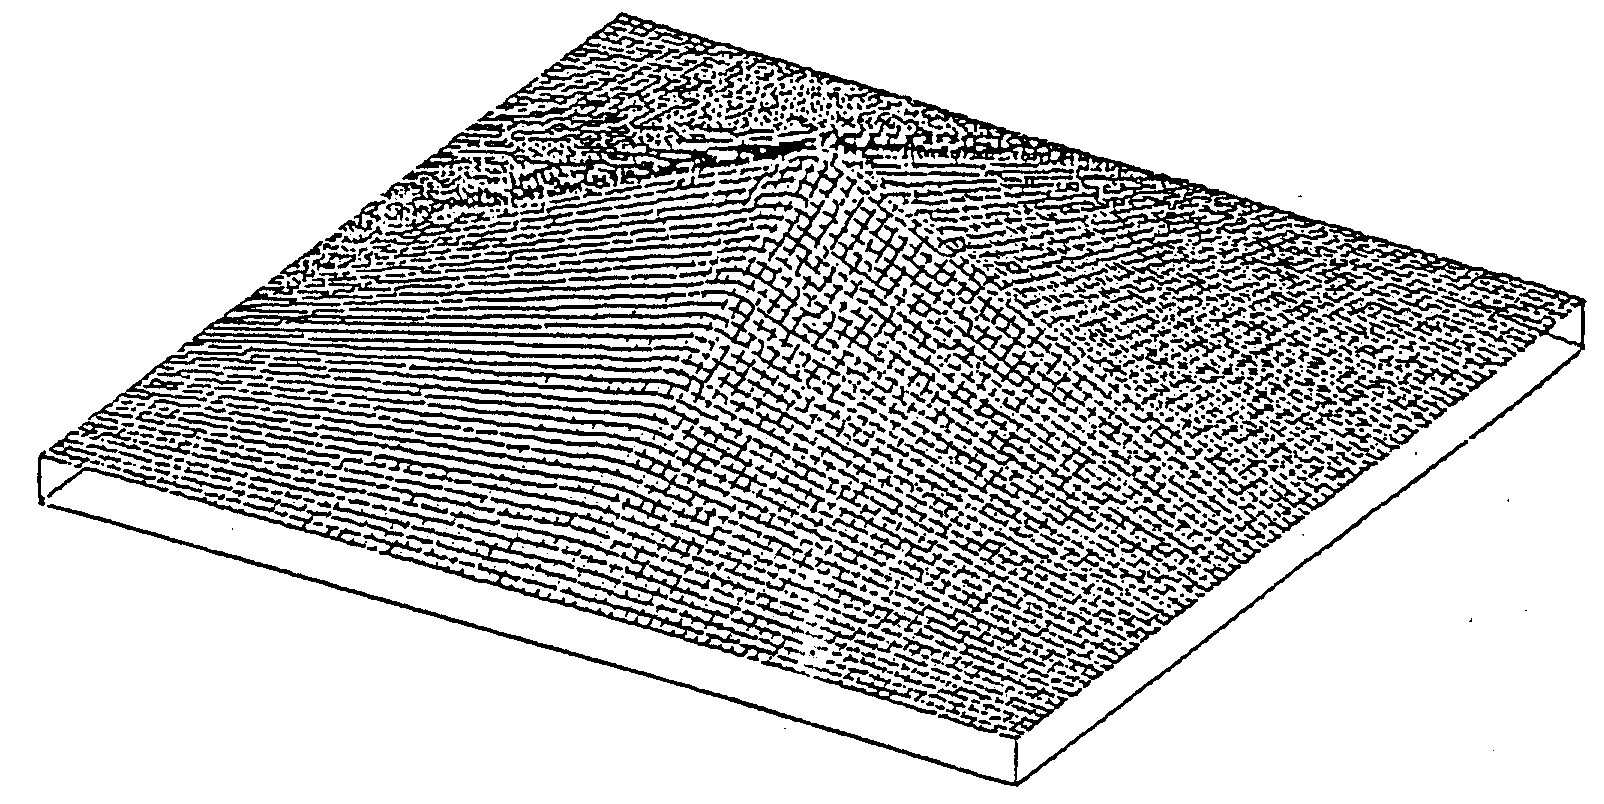
\includegraphics[width=0.45\textwidth]{images/bilinear_spline.jpg}
        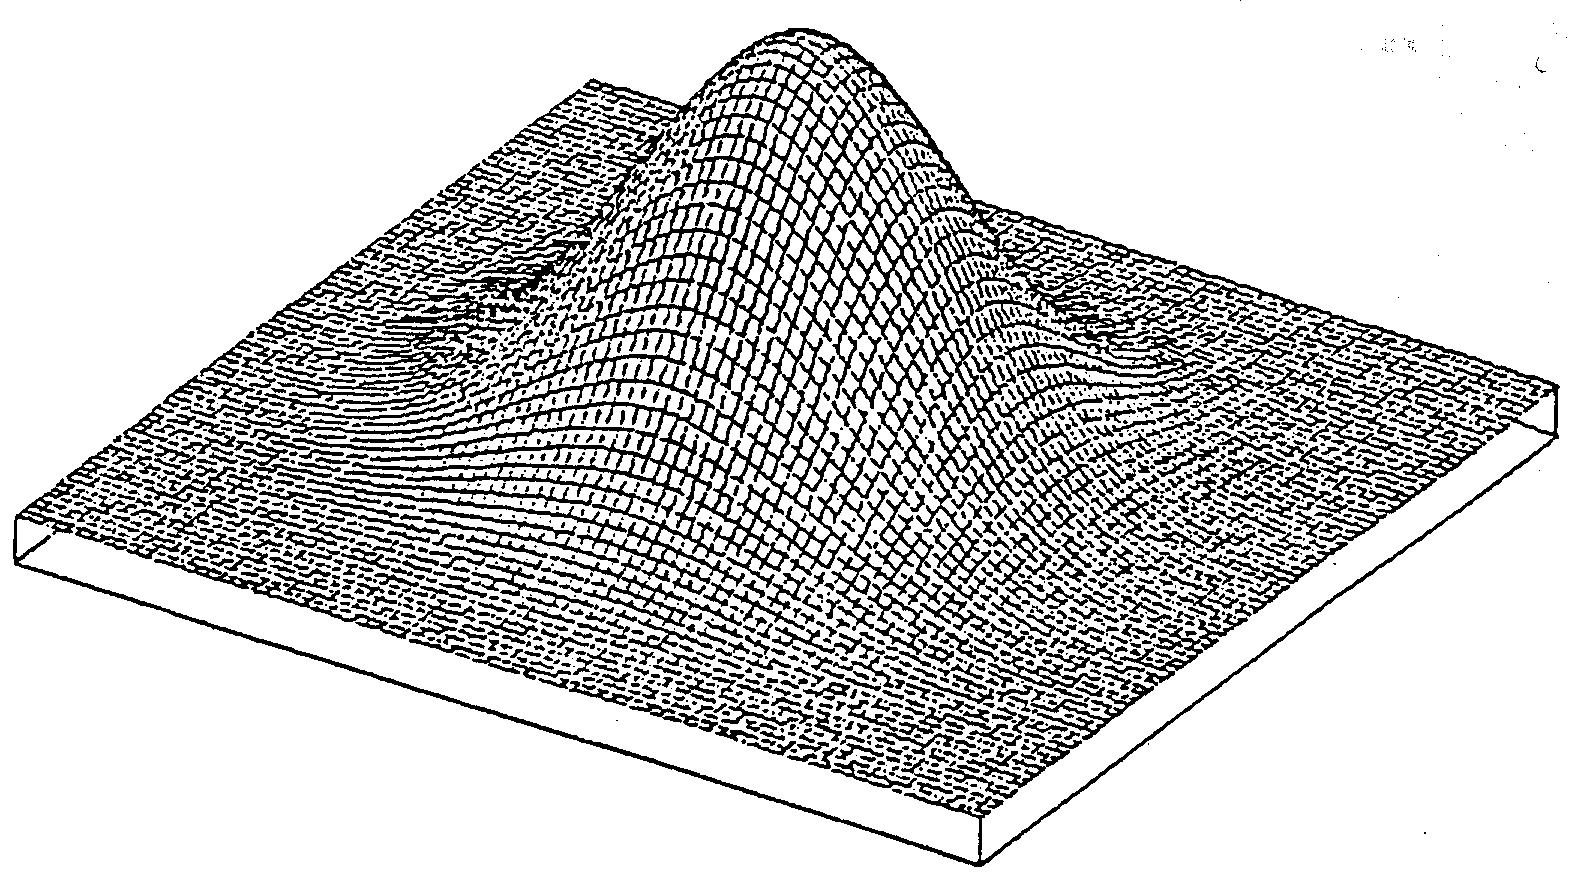
\includegraphics[width=0.45\textwidth]{images/bicubic_spline.jpg}
        %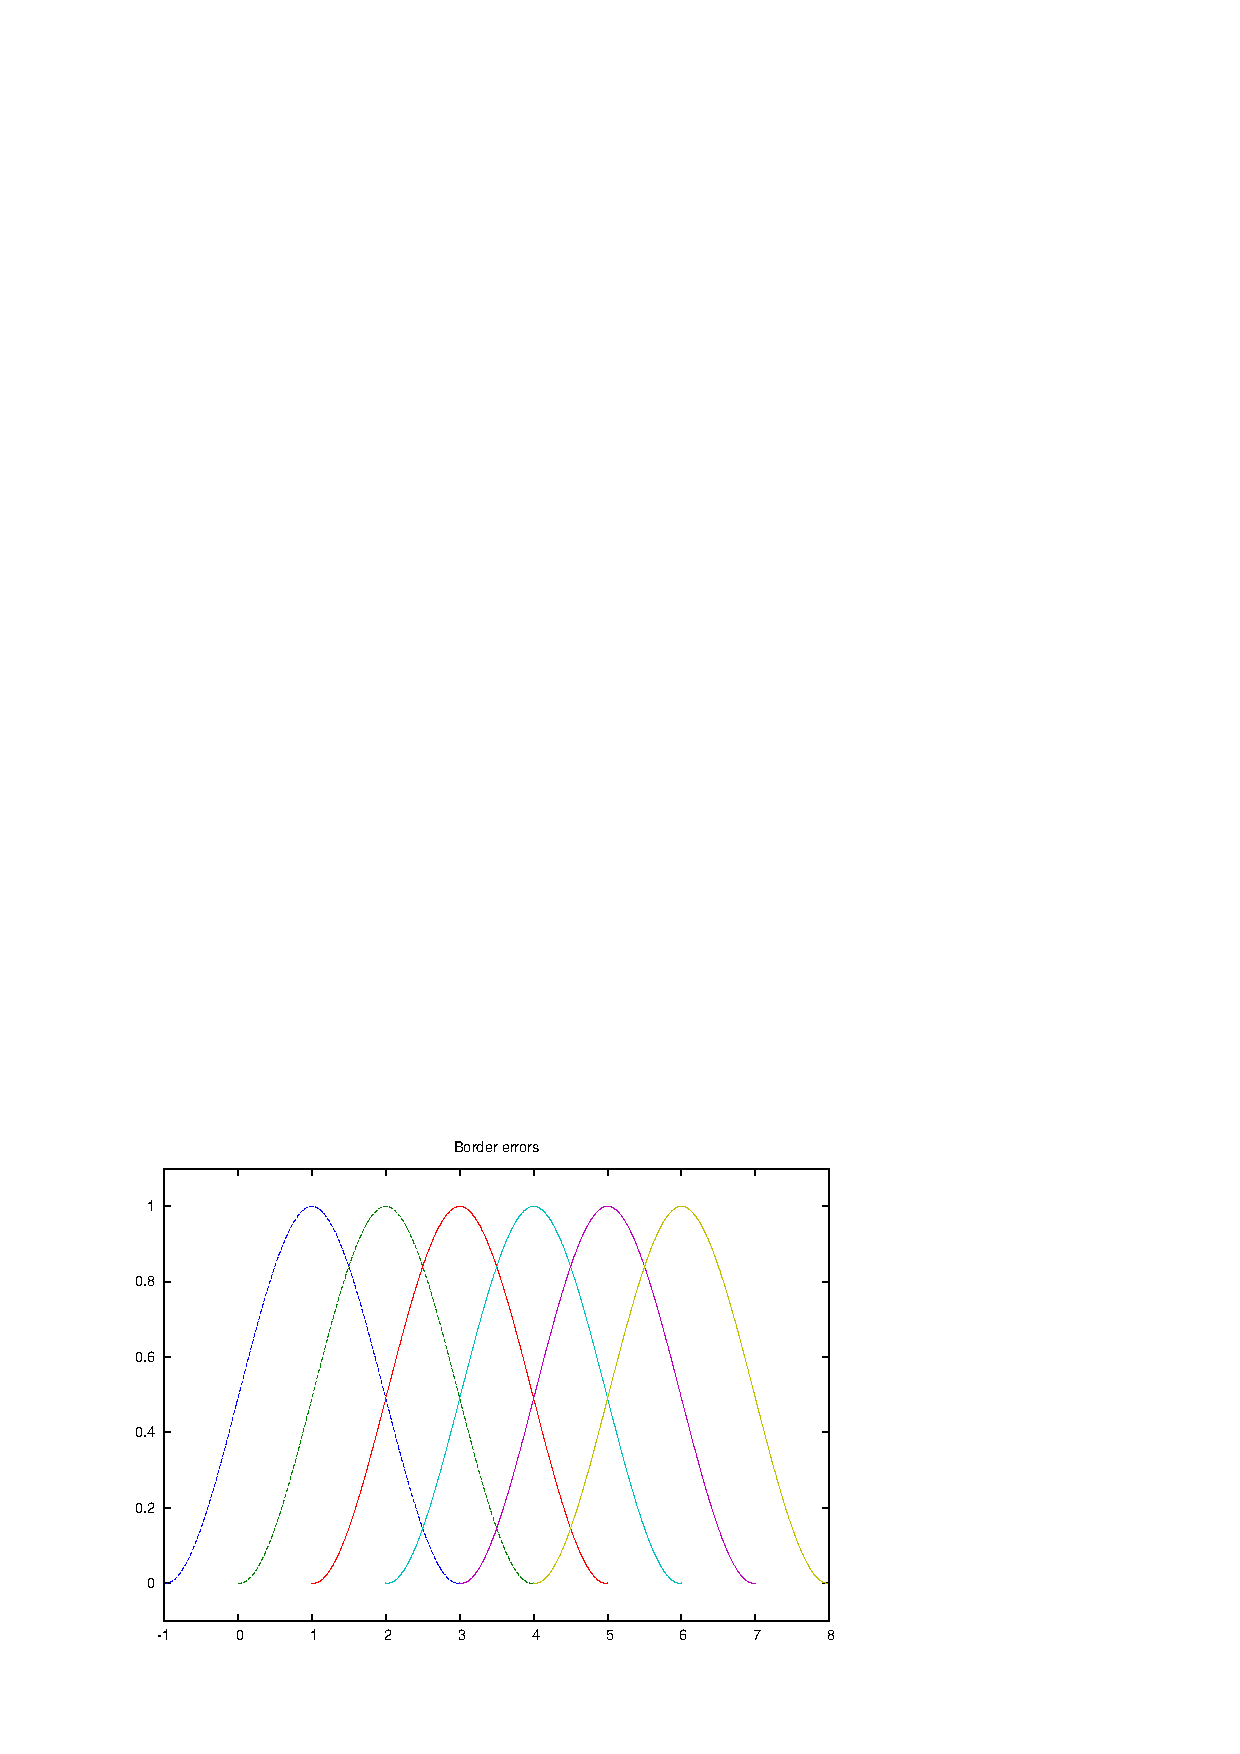
\includegraphics[width=0.45\textwidth]{images/border_errors.jpg}
    \end{center}
\end{frame}
%%==================================================================Sb
\subsection{Puntos groseros}
%%==================================================================F
\begin{frame}
   \frametitle{Puntos groseros}
   \begin{enumerate}
    \item Hay siempre puntos anómalos debido a diferentes eventos:
     \begin{itemize}
 	\item<2-> \alert<2,3,6>{Pájaros}
 	\item<4-> \alert<4,6>{Nubes de agua}
 	\item<5-> \alert<5,6>{``Multipath''}...
     \end{itemize}
    \item<6>{\alert<6>{\textexclamdown\textexclamdown Deben ser eliminados!!}} 
   \end{enumerate}
   \begin{picture}(0,100)
       \uncover<2>{\put(10,10){
\includegraphics[height=30mm]{images/angry_birds}}}     
       \uncover<3,6>{\put(10,10){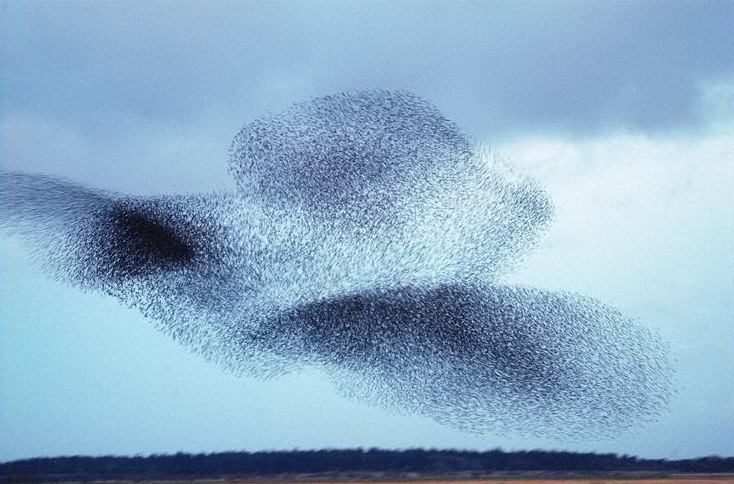
\includegraphics[height=30mm]{images/bandada}}}
       \uncover<4>{\put(50,10){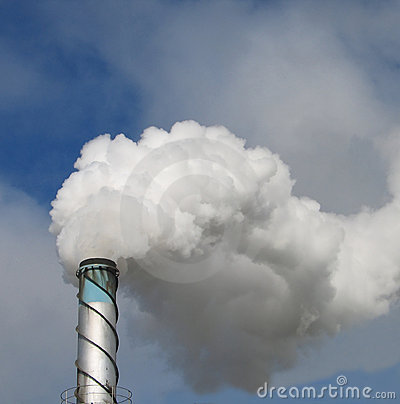
\includegraphics[height=30mm]{images/vapor_chimenea}}}
       \uncover<4,6>{\put(150,10){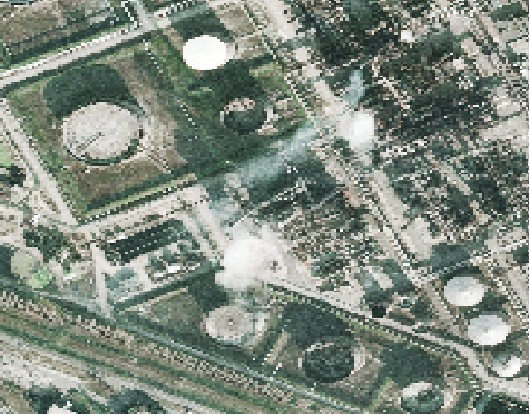
\includegraphics[height=30mm]{images/fumo}}}
       \uncover<5,6>{\put(280,10){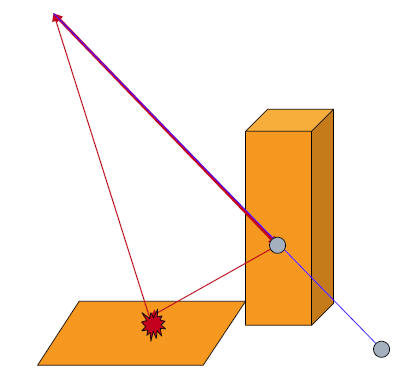
\includegraphics[height=30mm]{images/multipath}}}
    \end{picture}
\end{frame}
%%==================================================================F
\begin{frame}
   \frametitle{Detección de puntos groseros}
   \begin{itemize}
    \item<1-> La eliminación se hace mediante una interpolacion con splines 
        bicúbicas bastante lisa y baja resolución.
    \item<8-> Aquellos puntos que se alejen más de un umbral determinado son 
        considerados como puntos groseros y eliminados.
    \item<9-> El umbral por defecto son \alert<8>{$50~m$}
   \end{itemize}

    \begin{picture}(0,100)
       \only<2>{\put(80,0){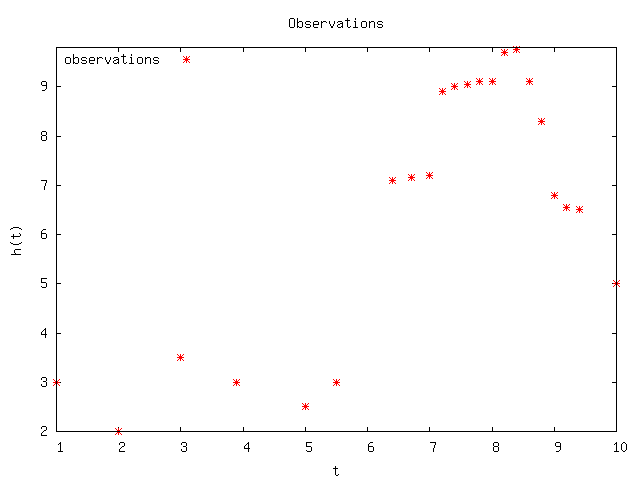
\includegraphics[height=35mm]{images/obs_splines}}}
       \only<3,8->{\put(80,0){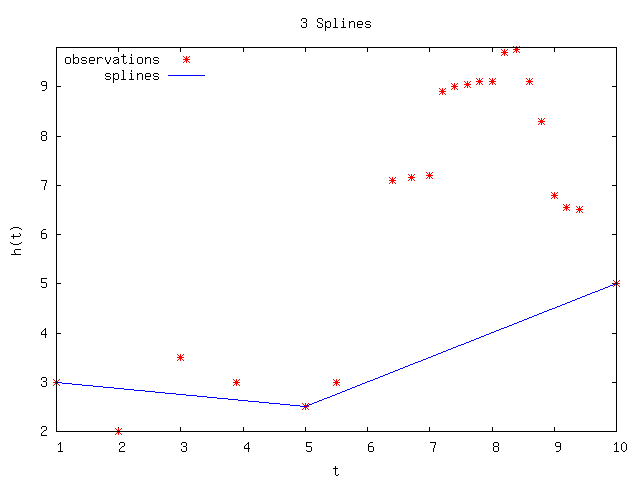
\includegraphics[height=35mm]{images/3splines}}}
       \only<4>{\put(80,0){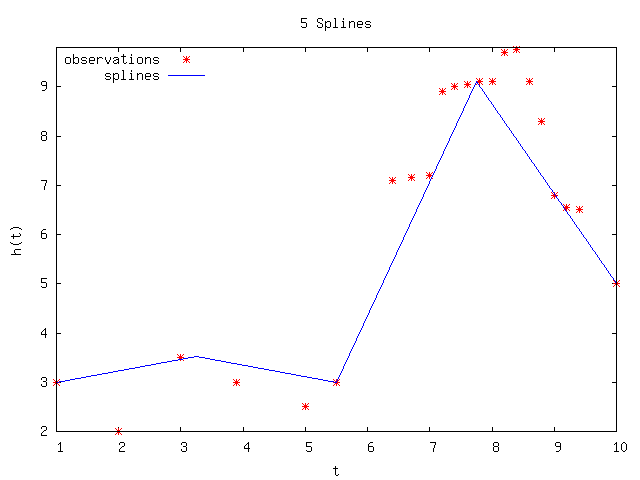
\includegraphics[height=35mm]{images/5splines}}}
       \only<5>{\put(80,0){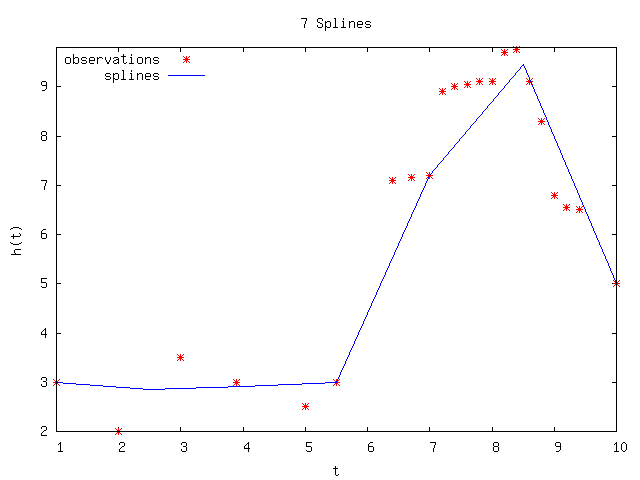
\includegraphics[height=35mm]{images/7splines}}}
       \only<6>{\put(80,0){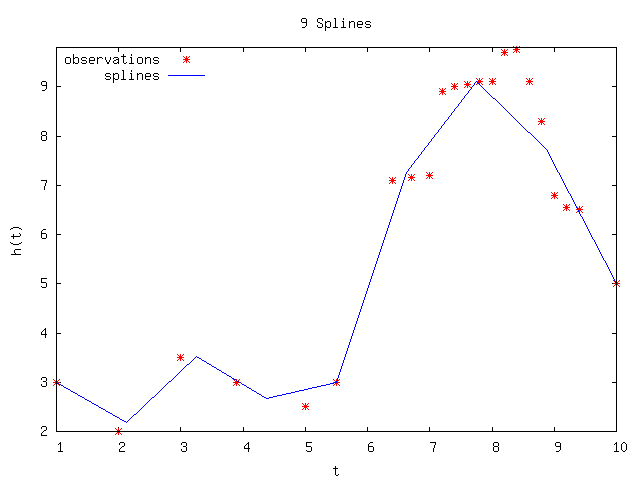
\includegraphics[height=35mm]{images/9splines}}}
       \only<7>{\put(80,0){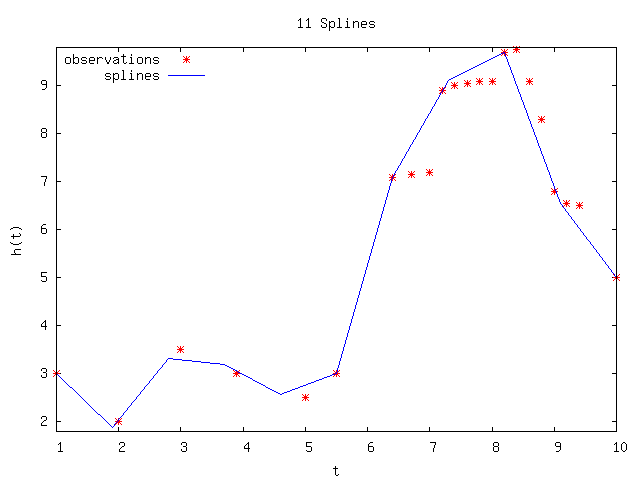
\includegraphics[height=35mm]{images/11splines}}}
    \end{picture}
\end{frame}
%%==================================================================Sb
\subsection{Detección de bordes}
%%==================================================================F
\begin{frame}
  \frametitle{Detección de bordes}
\begin{beamerboxesrounded}[shadow=true]{Definición: \emph{Borde}}
     \alt<1>{\alert<1>{NO} es un señor antipático $\Rightarrow$ \alert<1>{NO} 
        es tu jefe}{Es una fuerte variación en altura correspondiente a una 
        pequeña variación en planimetría}
    \end{beamerboxesrounded}

\only<2>{
  \begin{picture}(0,100)
    %\centering
    \begin{tikzpicture}[scale=0.7]
    \draw[thick] (-5,0) -- (2.5,0);
    \filldraw[black!20!white] (-2,0) -- (-2,2) -- (0,3) -- (2,2) -- (2,0) -- cycle;
    \draw (-2,0) -- (-2,2) -- (0,3) -- (2,2) -- (2,0) -- cycle;

    \coordinate[mark coordinate] (S) at (-2,0);
    \coordinate[mark coordinate] (B) at (-2,2);
    \node[anchor=south east] at (S){};
    \node[anchor=north west] at (B){};
    \node[anchor=west] at (-1,1){Objeto};
    \end{tikzpicture}
  \end{picture}
  \begin{picture}(0,100)
     \uncover<2>{\put(200,-5){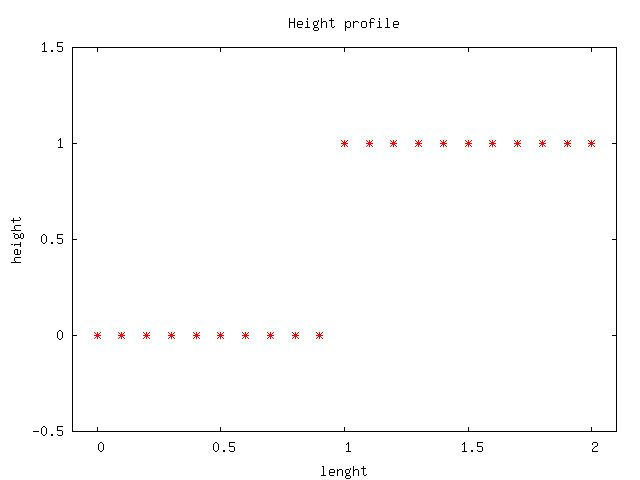
\includegraphics[height=30mm]{images/height_edge}}}
  \end{picture}
}
\begin{enumerate}
 \item<3-> El análisis de bordes no es fácil porque los puntos no están distribuidos regularmente
 \item<4-> Se pueden regularizar los puntos $\Rightarrow$ se rasteriza: 
    \begin{itemize}
        \item<4-> \alert<4>{mínimo} y \alert<4>{máximo}
	\item<5-> \alert<5>{Media}
	\item<6-> \alert<6>{Interpolación}
	\item<7-> \alert<7>{\emph{kriging}}...
    \end{itemize}
  \item<8-> \alert<8>{Pérdida de información} altimétrica
\end{enumerate}
\end{frame}
%%==================================================================F
\begin{frame}
  \frametitle{Cálculo de bordes}
\begin{enumerate}
  \item Se trabaja con una interpolación con spline bilineares que se ajuste 
    mucho a las observaciones (nuestros puntos)
  \item<2->{Para esta superficie se calcula:}
\begin{itemize}
 \item<2-> El \alert<2>{Gradiente} para cada punto: $G_m = \sqrt{G_x^2 + G_y^2} = \sqrt{\left( \dfrac{dz}{dx}\right)^2 + \left( \dfrac{dz}{dy}\right)^2}$
 \item<3-> La \alert<3>{dirección normal}: $\vartheta_P = \arctan\left(\dfrac{G_y}{G_x} \right)$
\end{itemize}
\end{enumerate}

  \uncover<4->{\alert<4>{Estos dos parámetros no son suficientes!!}}
\end{frame}
%%==================================================================F
\begin{frame}
  \frametitle{Valor gradiente}
  \begin{enumerate}[<+->]
   \item El gradiente tiene un valor muy alto en el borde de los objetos pero también el punto exterior más próximo
   \item Debido al ruido en las observaciones, el valor más alto del gradiente \alert<2>{puede ser el equivocado}
  \end{enumerate}
    \begin{picture}(0,110)
        \only<1>{\put(80,0){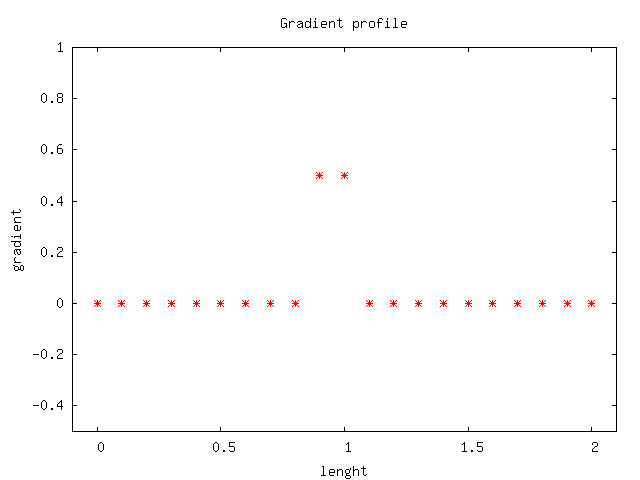
\includegraphics[height=40mm]{images/gradient_edge}}}
        \only<2>{\put(80,0){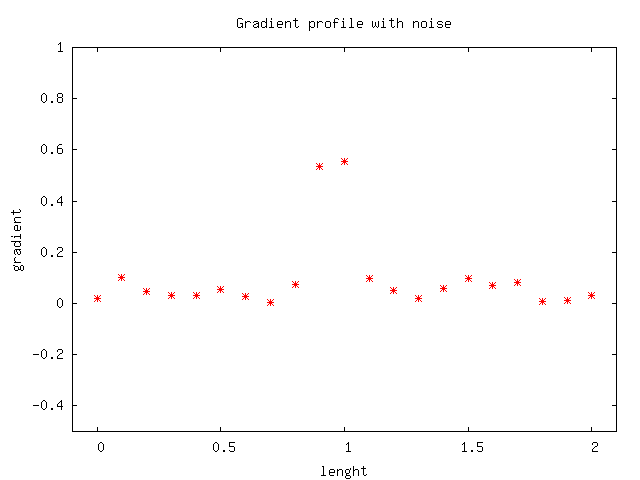
\includegraphics[height=40mm]{images/gradient_noise_edge}}}
    \end{picture}
\end{frame}
%%==================================================================F
\begin{frame}
  \frametitle{Cálculo de residuos}%
  \begin{enumerate}[<+->]%
   \item Se trabaja con una interpolación con spline bicúbicas con resolución muy baja 
       para obtener una \alert<1>{superficie muy lisa}%
   \item Se calcula el residuo entre la superficie y las observaciones%
   \item El punto con residuo positivo será nuestro punto \alert<3>{borde} %
  \end{enumerate}%
\uncover<3->{
  \begin{figure}[!b]
    \centering
    \begin{tikzpicture}[scale=0.85]
    %\includegraphics[height=50mm]{images/figure_6}
    \draw[thick] (-5,0) -- (3,0);
    \filldraw[black!20!white] (-2,0) -- (-2,2) -- (0,3) -- (2,2) -- (2,0) -- cycle;
    \draw (-2,0) -- (-2,2) -- (0,3)node[above]{Objeto} -- (2,2) -- (2,0) -- cycle;
    \draw[thick] (-4.5,0.3)node[above]{Interpolaci\'on} -- 
        (-3.5,0.3) .. controls (-1.5,.4) and (-1.5,2) .. (0,2);

    \coordinate[mark coordinate] (N) at (-2,0);
    \coordinate[mark coordinate] (P) at (-2,2);
    \node[anchor=south east] at (N){--};
    \node[anchor=north west] at (P){+};

    \node[anchor=west] at (-0.5,1){+ Borde};
    \node[anchor=west] at (-0.5,0.5){-- \  Terreno};
    \end{tikzpicture}
  \end{figure}
}
\end{frame}
%%==================================================================F
\begin{frame}
  \frametitle{Identificación final de bordes}%
  Para que un punto sea considerado como el borde de un objeto se debe cumplir:
  \begin{enumerate}[<+->]%
	\item El gradiente debe ser mayor que un cierto umbral dado por el usario
	\item Si el gradiente es grande pero \alert<2>{sin} llegar al umbral, además se debe verificar que:
	\begin{itemize}
	 \item El residuo es \alert<3>{positivo}
	 \item La dirección normal no se desvía mas de un valor dado.
	\end{itemize}
  \end{enumerate}
\end{frame}
%%==================================================================Sb
\subsection{Region Growing}
%%==================================================================F
\begin{frame}
  \frametitle{``Region Growing''}
\begin{beamerboxesrounded}[shadow=true]{Hipótesis}
El interior del objeto será siempre igual o más alto que los bordes (su altura media)
\end{beamerboxesrounded}

\begin{enumerate}
 \item El objetivo en este paso es reconocer el \alert{interior} de los objetos
 \item Para cada borde se construye un \alert{conj. convexo} y en su interior se ejecuta un algoritmo de \alert{\emph{region growing}} para verificar la hipótesis
\end{enumerate}
\end{frame}
%%==================================================================F
%\begin{frame}
%  \frametitle{``Region Growing''}
%\begin{figure}[t]
% \begin{center}
%\tiny
%  \begin{tikzpicture}[scale=0.2, node distance=1.25cm, auto]
%    % Region growing
%    \node[io] (semilla) {Elegir Semilla};
%    \node[block, below of=semilla] (este) {Moverse a celda Este};
%    \node[decision, below of=este] (visitadaE) {¿Visitada?};
%    \node[block, below of=visitadaE, node distance=1cm] (norte) 
%        {Moverse a celda Norte};
%    \node[decision, below of=norte] (visitadaN) {¿Visitada?};
%    \node[block, below of=visitadaN, node distance=1cm] (visitada) 
%        {Marcar como visitada};
%    \node[block, right of=visitada, node distance=2cm] (retroceder) {Retroceder};
%    \node[decision, right of=visitadaE, node distance=1.5cm] (valor1E) 
%        {¿Valor = 1?};
%    \node[decision, left of=visitadaN, node distance=1.5cm] (valor1N) 
%        {¿Valor = 1?};
%    \node[decision, above of=retroceder] (EsSemilla) {¿Es la semilla?};
%    \node[io, right of=EsSemilla, node distance=1.5cm] (convhull) 
%        {Crear soporte compacto};
%
%    % Flujo
%    \path[line] (semilla) -- node{}(este);
%    \path[line] (este) -- node{}(visitadaE);
%    \path[line] (visitadaE) -- node{si}(norte);
%    \path[line] (visitadaE) -- node{no}(valor1E);
%    \path[line] (valor1E) |- node[near start]{si}(este);
%    \path[line] (valor1E) |- node[near start]{no}(norte);
%    \path[line] (norte) -- node{}(visitadaN);
%    \path[line] (visitadaN) -- node{si}(visitada);
%    \path[line] (visitadaN) -- node{no}(valor1N);
%    \path[line] (valor1N) |- node[near start]{si}(este);
%    \path[line] (valor1N) |- node[near start]{no}(visitada);
%    \path[line] (visitada) -- node{}(retroceder);
%    \path[line] (retroceder) -- node{}(EsSemilla);
%    \path[line] (EsSemilla) -- node[near start]{si}(convhull);
%    \path[line] (EsSemilla) |- node[near start]{no}(este);
%    \path[line] (convhull) |- node{}(semilla);
%  \end{tikzpicture}
% \end{center}
%\end{figure}
%\end{frame}
%%==================================================================F
\begin{frame}
  \frametitle{Primera clasificación}
Los puntos viene clasificados por su posición con respecto al terreno: \pause
\begin{enumerate}
 \item \alert{Objeto}: Si están dentro del conj. convexo y su altura es mayor que la altura media del borde
 \item \alert{Terreno}: En cualquier otro caso.
\end{enumerate}

\pause
Y por el tipo de impulso:
\begin{enumerate}
 \item \alert{\'Unico impulso}: Si solo se ha recibido un eco de ese punto
 \item \alert{Doble impulso}: Si se han recibido más impulsos
\end{enumerate}
\end{frame}
%%==================================================================Sb
\subsection{Corrección}
%%==================================================================F
\mode<beamer>{
  \pgfdeclareimage[width=0.4\textwidth]{fumo}{images/fumo}
  \pgfdeclareimage[width=0.4\textwidth]{fumo}{images/google_techos}
}
\begin{frame}
  \frametitle{Errores en la clasificación}
  \begin{columns}
    \begin{column}{0.5\textwidth}
      \begin{enumerate}[<+->]
    	\item La hipótesis de las alturas falla
        \item Confusión de alturas
    	\item Se han identificado bordes pertenecientes al terreno pero no a objetos
     \end{enumerate}
    \end{column}
   \begin{column}{0.45\textwidth}
   \begin{figure}[h!]
   \centering
      \only<1>{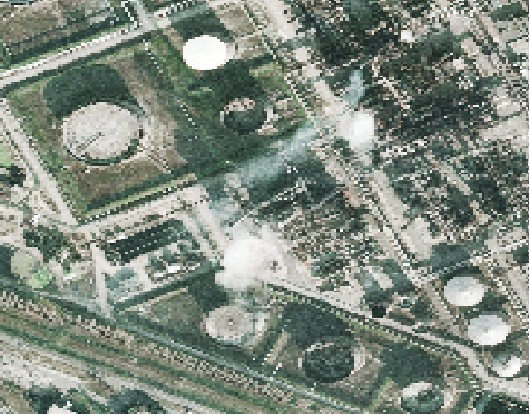
\includegraphics[height=40mm]{images/fumo}}
      \only<2>{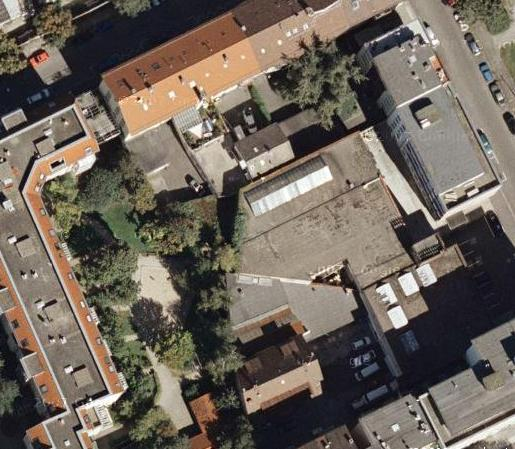
\includegraphics[height=40mm]{images/google_techos}}
      \only<3>{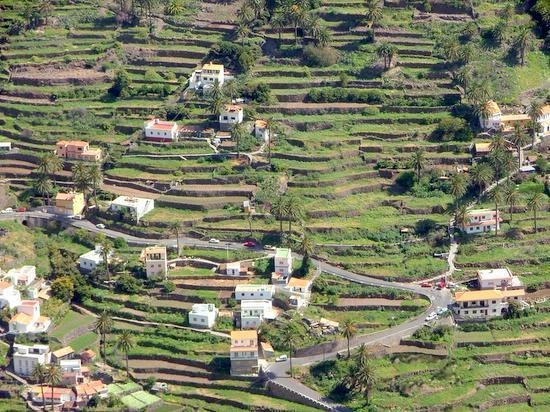
\includegraphics[height=40mm]{images/terrazas}}
   \end{figure}
   \end{column}
  \end{columns}
\end{frame}
%%==================================================================F
\begin{frame}
  \frametitle{Corrección final}
Se utilizan los puntos \alert<1>{Terreno único impulso} para realizar una
interpolación con splines bilineares y resolucion baja para obtener una
superficie bastante lisa.
  \begin{minipage}{0.5\textwidth}
    \begin{enumerate}
      \item<2-> Si un punto terreno está lo suficientemente alejado de la superficie se reclasifica como \alert<2>{objeto}
      \item<3-> Si un punto objeto está lo suficientemente cercano a la superficie se reclasifica como \alert<3>{terreno}
    \end{enumerate}
  \end{minipage}%
  ~%
  \begin{minipage}{0.45\textwidth}
   \begin{figure}[h!]
   \centering
      \uncover<2->{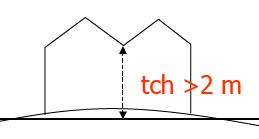
\includegraphics[height=20mm]{images/correct_objeto}}
      \uncover<3->{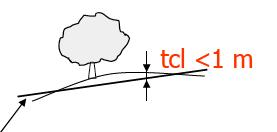
\includegraphics[height=20mm]{images/correct_terreno}}
   \end{figure}
  \end{minipage}
\end{frame}
%%==================================================================Sb
\subsection{Vegetación}
%%==================================================================F
\begin{frame}
  \frametitle{Motivaciones}
  \begin{enumerate}[<+->]
    \item El filtro anterior clasifica entre \alert{terreno} Vs. \alert{objeto}: 
  \begin{itemize}[<+->]
    \item Participó en el test del ISPRS: Buenos resultados
    \item Incompleta: \alert<3>{NO distingue vegetación}
  \end{itemize}
    \item Detectar vegetación en una nube ALS es importante para
      \uncover<4->{\alert{estudios hidrológicos}},
      \uncover<5->{\alert{modelización urbana},} \uncover<6->{\alert{estudios
      forestales}, etc\ldots}
    \item Desarrollo del filtro de vegetación porque:
    \begin{itemize}[<+->]
    \item Existe ya una estructura adecuada de datos
    \item Dado que está bajo licencia libre, su publicación también deberá ser
      libre
    \item Completar el algoritmo que participó en el ISPRS
    \end{itemize}
\end{enumerate}
\end{frame}
%%==================================================================F
\begin{frame}
  \frametitle{Clasificación de vegetación}
  \begin{enumerate}
    \item<1-> Los datos de partida son los clasificados como terreno u objecto
    (tanto único como doble impulso).
    \item<2-> Se crea una máscara ráster.
    \item<3-> Podemos buscar:
      \begin{enumerate}
        \item<3-> \alert<3>{Edificios}
          \begin{itemize}
            \item valor celda = 1 si al menos un punto ``objeto único impulso''
              cae en ella.
            \item valor de celda = 0 en otro caso
          \end{itemize}
        \item<4-> \alert<4>{Vegetación}
          \begin{itemize}
            \item valor celda = 1 si al menos un punto ``terreno doble impulso''
              cae en ella.
            \item valor de celda = 0 en otro caso
          \end{itemize}
      \end{enumerate}
  \end{enumerate}
\end{frame}
%%==================================================================F
\begin{frame}
  \frametitle{Clasificación de vegetación}
  \begin{enumerate}
    \item<1-> Se aplica un algoritmo de ``region growing'' a la mascara raster
        para crear conj. convexos. 
      \item<2-> Las \alert<2>{dimensiones} y la relación \alert<2>{área/perímetro}
        se usan para la clasificación de los segmentos:
    \begin{itemize}
        \item Objetos pequeños o muy estrechos no son edificios
        \item Puntos ``terreno doble impulso'' son considerados como vegetación
        \item Puntos ``objeto doble impulso'' fuera de los segmentos son
          considerados como vegetación
        \item El resto siempre es considerado edificio
    \end{itemize}
  \end{enumerate}
\end{frame}
%%==================================================================F
\begin{frame}
  \frametitle{Árbol de clasificación del filtro vegetación}
\begin{figure}[t!]
\begin{center}
\scriptsize
\begin{tikzpicture}[scale=0.75,grow=right, sloped,
    level 1/.style={sibling distance = 3cm, level distance = 3cm}, 
    level 2/.style={sibling distance = 1.5cm, level distance = 3cm},
    level 3/.style={sibling distance = 0.75cm, level distance = 2.5cm},
    punto/.style={text width=7em, text centered},
    mascara/.style={text centered, text width=5em},
    end/.style={circle, minimum width=3pt,fill, inner sep=0pt}]
  \node {Punto}
    child{ node[punto] {Terreno único impulso} 
       child{ node [end, label=right:{\textbf{Terreno}}] {}
              edge from parent node[above] {\scriptsize{Siempre}}
       }
    }
    child{ node[punto] {Terreno doble impulso}
       child{ node[mascara] {Máscara Terreno} 
          child{ node [end, label=right:{\textbf{Terreno}}] {}
                 edge from parent node[below] {\scriptsize{Fuera}}
          }
          child{ node [end, label=right:{\textbf{Vegetación}}] {}
                 edge from parent node[above] {\scriptsize{Dentro}}
          }
       }
       child{ node[mascara] {Máscara Objeto}
          child{ node [end, label=right:{\textbf{Vegetación}}] {}
                 edge from parent node[above] {\scriptsize{Siempre}}
          }
       }
    }
    child{ node[punto] {Objeto doble y único impulso}
       child{ node[mascara] {Máscara Terreno} 
          child{ node [end, label=right:{\textbf{Objeto}}] {}
                 edge from parent node[below] {\scriptsize{Fuera}}
          }
          child{ node [end, label=right:{\textbf{Vegetación}}] {}
                 edge from parent node[above] {\scriptsize{Dentro}}
          }
       }
       child{ node[mascara] {Máscara Objeto}
          child{ node [end, label=right:{\textbf{Vegetación}}] {}
                 edge from parent node[below] {\scriptsize{Fuera}}
          }
          child{ node [end, label=right:{\textbf{Objeto}}] {}
                 edge from parent node[above] {\scriptsize{Dentro}}
          }
       }
    }
;
\end{tikzpicture}
\caption{Árbol de decisión para la clasificación de los puntos en terreno,
vegetación y edificio.}
\label{fig:decision_tree}
\end{center}
\end{figure}
\end{frame}
%%==================================================================F
\begin{frame}
  \frametitle{Clasificación de la vegetación}
  \begin{minipage}{0.45\textwidth}
    \begin{figure}[h!]
      \centering
      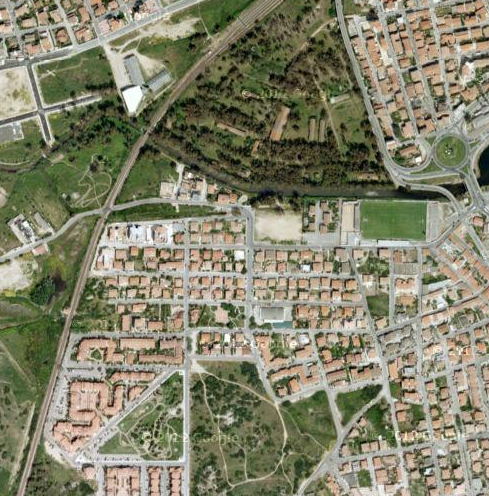
\includegraphics[width=0.95\textwidth]{images/olbia}
    \end{figure}
  \end{minipage}
  \begin{minipage}{0.45\textwidth}
    \begin{figure}[h!]
      \centering
      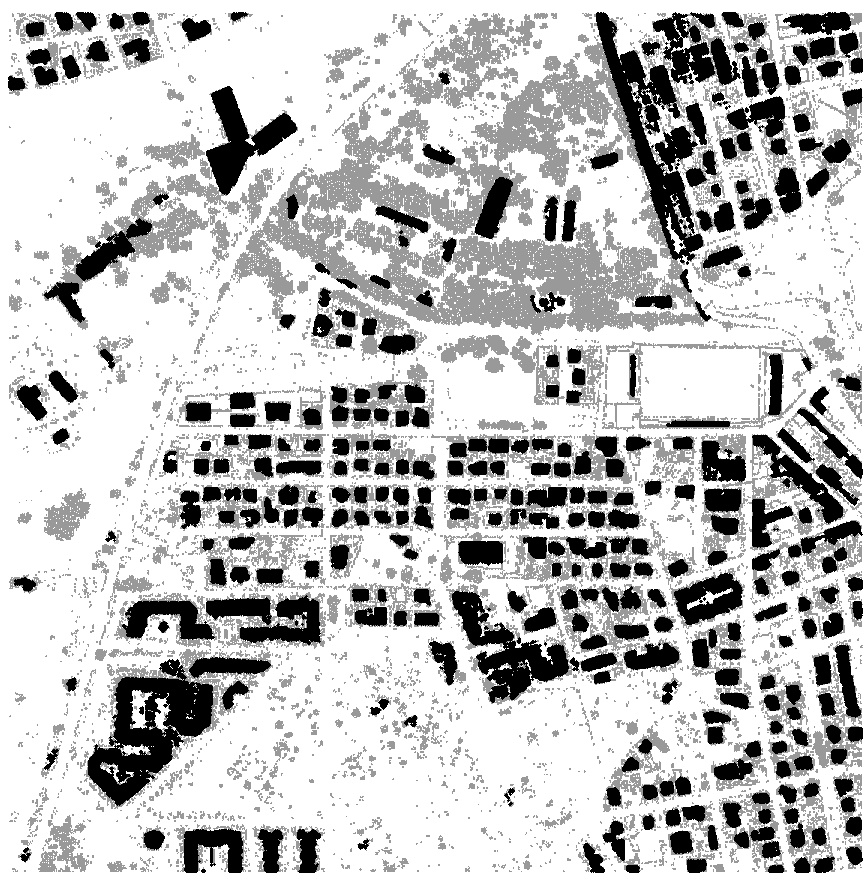
\includegraphics[width=0.95\textwidth]{images/olbia_veg_build}
    \end{figure}
  \end{minipage}
\end{frame}
%%==================================================================F
\begin{frame}
  \frametitle{Resultados}
  \begin{enumerate}[<+->]
    \item El filtro vegetación está fuertemente afectado por el filtro terreno:
    \begin{itemize}
      \item Altos errores del tipo I (error de omisión) debido
        a bordes de edificios mal clasificados como vegetación.
      \item Errores de tipo II (error de comisión) debido
        a zonas de densa vegetación tomada como edificios o incluso zonas
        terreno clasificadas como objetos.
    \end{itemize}
    \item Alrededor del 90\% de los puntos se clasifican correctamente.
    \begin{itemize}
      \item Amplias zonas vegetales son correctamente clasificadas, así como la
        mayoría de árboles individuales. 
      \item La figura y forma de los eficios está siempre bien definida.
    \end{itemize}
  \end{enumerate}
\end{frame}
%%==================================================================F
\begin{frame}
  \frametitle{Resultados}
  \begin{itemize}[<+->]
    \item Errores de \alert<1>{tipo I} (descartar puntos edificio):
      \alert<1>{$16.6\%$}
    \item Errores de \alert<2>{tipo II} (Aceptar puntos vegetación como
      edificio): \alert<2>{$7.5\%$}
      \item \alert<3>{Error Total}: \alert<3>{$10.6\%$}
    \end{itemize} 
     \begin{table}[b!]
    \centering
    \begin{tabular}{lccccr}
      \multicolumn{6}{c}{\bfseries{Matriz de Confusión}} \\
      \hline
      \textbf{Clasif.} & \multicolumn{2}{c}{Edificios} & 
        \multicolumn{2}{c}{Vegetación} & Total \\
      \cline{2-6}
      \textbf{Verdad} & \multicolumn{2}{c}{Puntos (\%)} & 
        \multicolumn{2}{c}{Puntos (\%)} & Total \\
      \hline
      Edif. & \multicolumn{2}{c}{179678 (83.4)} & 
        \multicolumn{2}{c}{34919 (\alert<1>{16.6})} & 214597 \\
      Veg. & \multicolumn{2}{c}{37590 (\alert<2>{7.5})} & 
        \multicolumn{2}{c}{388709 (92.5)} & 426299 \\
      Total & \multicolumn{2}{c}{217268 (--)} & 
      \multicolumn{2}{c}{423628 (--)} & 640896\footnote{Las estadísticas están referidas a aquellos puntos con una pre-clasificación distinta de terreno único impulso} \\
      \hline
    \end{tabular}
    \end{table}
\end{frame}
%%==================================================================F
\begin{frame}
  \frametitle{Solapes}
  \begin{enumerate}
    \item<1-> Durante las interpolaciones, se divide toda la región en teselas
      solapadas
      \begin{itemize}
        \item<1-> Permite la computación de la interpolación de modo más rápido
        \item<2-> Elimina los problemas de alocación de memoria
      \end{itemize}
    \item<3-> En las zonas de solape
    \begin{itemize}
        \item<3-> Asegura la continuidad de toda la interpolación
        \item<4-> Introduce una discontinuidad en la primera derivada: Errores en el
          mapa de aspectos en zonas con ausencia de datos
      \end{itemize}
  \end{enumerate}
\end{frame}
%%==================================================================F
\begin{frame}
  \frametitle{Solapes}
    \begin{figure}[h!]
      \centering
      \only<1>{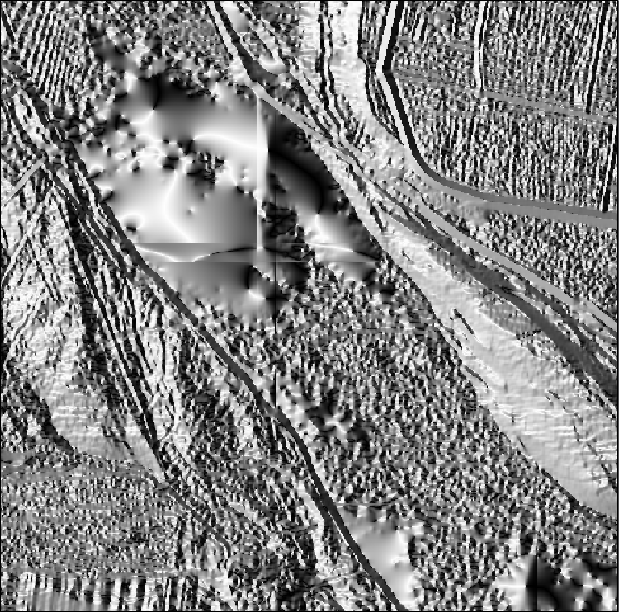
\includegraphics[width=0.65\textwidth]{images/errores_aspect}}
      \only<2>{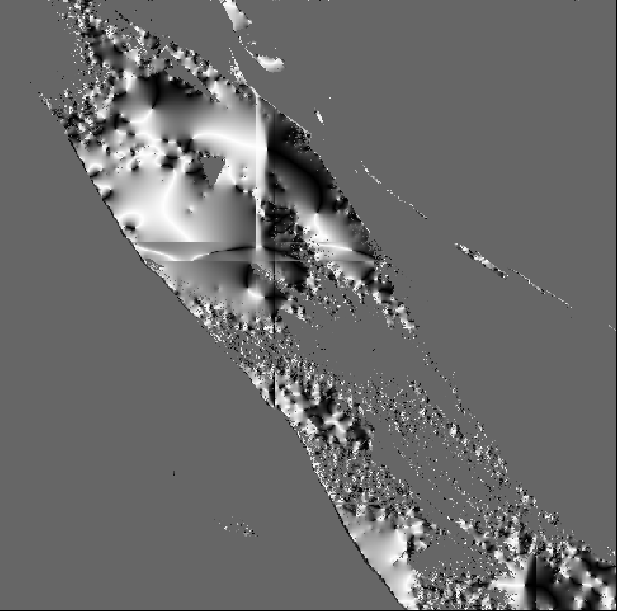
\includegraphics[width=0.65\textwidth]{images/errores_aspect_mascara}}
      \only<3>{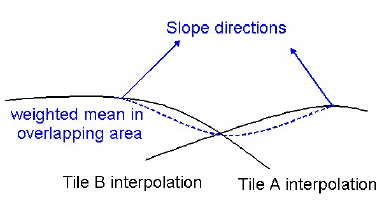
\includegraphics[width=0.65\textwidth]{images/error_interpolacion_solapes}}
    \end{figure}
\end{frame}
%%==================================================================F
\begin{frame}
  \frametitle{Computación}
    \begin{table}[h!]
      \centering
    \begin{tabular}{ccrrr}
    \toprule
    \multicolumn{5}{c}{\bfseries Interpolación Bilinear} \\
    \hline
    \bfseries Paso de Spline & \bfseries Número de teselas & \bfseries
    tradicional & \bfseries teselado & \bfseries gain \\ 
    % (m) & (NSxEW) & (time) & (time) & \\
    \hline\hline
    1 & 16x16 & 2h16m42s & 1h33m47s & 31,4\% \\ 
    2 & 8x8 & 32m33s & 22m18s & 31,5\% \\ 
    4 & 4x4 & 8m03s & 6m10s & 23,4\%\\ 
    8 & 2x2 & 2m18s & 2m30s & -8,7\% \\
    16 & 1x1 & 1m01s & 1m41s & -65,6\% \\
    \bottomrule
    \end{tabular}
    \end{table}
\end{frame}
%%==================================================================F
\begin{frame}
  \frametitle{Solapes}
    \begin{figure}[h!]
\centering
\begin{tikzpicture}[scale=0.50]
  \filldraw[fill=gray!40!white]   
    (4,0) -- (4,5) -- (9,5) -- (9,0) -- cycle;
  \draw (0,0) -- (0,5) -- (5,5) -- (5,0) -- cycle;
  \draw
    (0,4) node[anchor=north west] {Tesela 3} -- 
    (0,9) node[anchor=north west] {Tesela 1} -- 
    (5,9) node[anchor=north west] {Tesela 2} -- 
    (5,4) node[anchor=north west] {Tesela 4} -- cycle;
  \draw (4,4) -- (4,9) -- (9,9) -- (9,4) -- cycle;
  \draw
    (0,5) -- (4,5) -- node[below=.1cm] {1} 
    (5,5) -- node[below=0.1cm] {2} 
    (8,5) -- node[below=0.1cm] {3} (9,5); 
  \draw
    (0,1) -- (4,1) -- node[below=.1cm] {7} 
    (5,1) -- node[below=.1cm] {8} 
    (8,1) -- node[below=.1cm] {9} (9,1); 
  \draw
    (0,4) -- (4,4) -- node[below=.75cm] {4} 
    (5,4) -- node[below=.75cm] {5} 
    (8,4) -- node[below=.75cm] {6} (9,4); 
  \draw (4,0) -- (4,9); 
  \draw (8,0) -- (8,9); 
    % Continuacion de teselas en lineas de puntos
  \draw[thick] (4,0) -- (4,5) -- (9,5) -- (9,0) -- cycle;
  \draw[dotted,thick] (9,0) -- (10,0);
  \draw[dotted,thick] (9,1) -- (10,1);
  \draw[dotted,thick] (9,4) -- (10,4);
  \draw[dotted,thick] (9,5) -- (10,5);
  \draw[dotted,thick] (9,9) -- (10,9);
  \draw[dotted,thick] (0,-1) -- (0,0);
  \draw[dotted,thick] (4,-1) -- (4,0);
  \draw[dotted,thick] (5,-1) -- (5,0);
  \draw[dotted,thick] (8,-1) -- (8,0);
  \draw[dotted,thick] (9,-1) -- (9,0);
    \end{tikzpicture}
    \end{figure}
\end{frame}
%%==================================================================F



%%==================================================================FRONT PAGE AND TOC
%% For article only
%\mode<presentation:0>{\thispagestyle{empty}\maketitle}
%
%% For presentation only
%\mode<presentation| article:0| handout:0>{
%    \begin{frame}<article:0>[label=portada]
%    \titlepage
%    \end{frame}%Fin del frame
%}
%
%% For handout only
%\mode<handout>{
%  \begin{frame}[label=portada]
%    \maketitle
%  \end{frame}
%}
%
%%% TABLE OF CONTENTS
%\begin{frame}[label=toc]
%    \mode<article:0>{\frametitle{Contents}}
%    \mode<presentation>{\small}
%    \tableofcontents%[hidesubsections]
%\end{frame}
%
%%==================================================================S LOS DATOS
\section{Los datos}
%%==================================================================F 
\begin{frame}
\frametitle{La nube de puntos}
Metadatos
\begin{itemize}
 \item Sensor LiDAR: \alert{Optech ATLM}
 \item Datos disponibles: Primer y último impulso.
 \item Localización: Centro de Stuttgart (estación f.c.)
 \item Resolución: $0.91$ puntos$/m^2$; 
 \item Resolución media: $0.87$ puntos$/m^2$
 \item Numero de puntos: 
  \begin{enumerate}
    \item $259030$ de primeros retornos
    \item $259030$ de últimos retornos
   \end{enumerate}
\end{itemize}
\end{frame}
%%==================================================================F 
\pgfdeclareimage[width=0.5\textwidth]{stuttgart}{images/stuttgart}
\begin{frame}
\frametitle{Estación f.c. de Stuttgart}
 \begin{columns}
  \begin{column}{0.45\textwidth}
	Coordenadas UTM (MBR):
	\begin{itemize}
	 \item Norte = $5403764~m$
	 \item Sur = $5403188~m$
	 \item Oeste = $513632~m$
	 \item Este = $513118~m$
	\end{itemize}
   \end{column}
  \begin{column}{0.55\textwidth}
    \begin{center}
	\begin{tikzpicture}
    	  \pgftext[bottom,left,at={\pgfpointxy{0}{0}}]{\pgfuseimage{stuttgart}}
	\end{tikzpicture}
	\tiny{\textcopyright 2008 Google -- imágenes}
    \end{center}
   \end{column}
 \end{columns}
\end{frame}
%%==================================================================F 
\pgfdeclareimage[width=0.7\textwidth]{las}{images/las_format}
\begin{frame}
\frametitle{Estandard binario \emph{LAS} del ASPRS:}
\begin{itemize}
 \item Encabezado público
 \item Registros de longitud variable
 \item Puntos: X, Y, Z, Intensidad, clasificación, dirección de la pasada del vuelo,...
    \begin{center}
	\begin{tikzpicture}
    	  \pgftext[bottom,left,at={\pgfpointxy{0}{0}}]{\pgfuseimage{las}}
	\end{tikzpicture}
   \end{center}
 \item Para un conversor \alert{abierto} del estándar \emph{LAS}:
\beamergotobutton{\url{http://liblas.org/}}
\end{itemize}
\end{frame}
%%==================================================================F 
\frame[containsverbatim]{%
\frametitle {Posible formato ASCII}
\begin{center}
\begin{verbatim}
              X          Y       Z
          513628.82|5403190.04|291.40
          513628.85|5403191.47|291.24
          513628.95|5403192.93|294.31
          513628.99|5403194.45|294.17
          513628.97|5403196.05|291.26
          513629.01|5403197.58|291.24
          513629.05|5403199.10|291.25
          513629.09|5403200.53|291.26
                        ...
\end{verbatim}
\end{center}
}
%%==================================================================S
\section{Análisis LiDAR en GRASS}
%%==================================================================Sb
\begin{frame}
    \frametitle{Geographic Resources Analysis Support System\hfill 
\includegraphics[width=0.7cm]{images/grasslogo_transp_big.png}} 
     \begin{itemize}
	\item Conocido como \alert<1>{GRASS}: GIS para manipulación y análisis de datos geoespaciales.
	\item Como es un programa de \alert{códico abierto} con un montón de librerias, es muy adecuado para la implementación de nuestras propias herramientas.
	\item Escrito en C/C++, lo que permite implementar programas computacionalmente pesados $\Rightarrow$ \alert{ideal} para trabajar con LiDAR.
	\item GRASS $\geq$ 6 incluye indexación topológica $\Rightarrow$ \alert{fatal} para trabajar con LiDAR.
	\item Hay versiones para GNU/Linux, MS-Windows, Mac-OSX, SUN, etc. \alert{\textexclamdown\textexclamdown Todos lo pueden utilizar!!}
	\item Más información en:
	\beamergotobutton{\url{http://grass.osgeo.ogr}} 
    \end{itemize}
\end{frame}
%%==================================================================Sb
\subsection{Importando nube de puntos}
%%==================================================================F 
\begin{frame}[fragile,shrink=5]
 \frametitle{Importar como raster: \LARGE\path{r.in.xyz}}
\begin{verbatim}
GRASS6 (stuttgart): > # Primero conocemos la extensión del archivo
GRASS6 (stuttgart): > r.in.xyz -sg in=
GRASS6 (stuttgart): > # Fijo la región con la que trabajar
GRASS6 (stuttgart): > g.region n= s= e= w=
GRASS6 (stuttgart): > # Genero una visualización de las pasadas
GRASS6 (stuttgart): > # considerando para cada celda el número de puntos
GRASS6 (stuttgart): > r.in.xyz in= out=pasadas method=n fs='|'
\end{verbatim}
\end{frame}
%%==================================================================F 
\begin{frame}
 \frametitle{Solape de pasadas: \LARGE\path{r.in.xyz}}
\begin{verbatim}
GRASS6 (stuttgart): > # Genero un raster con la información LiDAR
GRASS6 (stuttgart): > r.in.xyz in= out=stuttgart fs='|'
\end{verbatim}
\end{frame}
%%==================================================================F 
\begin{frame}
 \frametitle{Importar como vectorial: \LARGE\path{v.in.ascii}}
\begin{verbatim}
GRASS6 (stuttgart): > # Genero dos vectoriales con la información LiDAR
GRASS6 (stuttgart): > # de último y primer impulso
GRASS6 (stuttgart): > v.in.ascii -tbzr in= out=stuttgart_first fs='|' z=3
GRASS6 (stuttgart): > v.in.ascii -tbzr in= out=stuttgart_last fs='|' z=3
\end{verbatim}
\end{frame}
%%==================================================================F 
\begin{frame}
 \frametitle{Importar como .LAS: \LARGE\path{v.in.las}}
\begin{verbatim}
GRASS6 (stuttgart): > v.in.lidar -p input=
GRASS6 (stuttgart): > v.in.lidar -i input="Serpent Mound Model LAS Data.las" location=
GRASS6 (stuttgart): > v.in.lidar -tb input="Serpent Mound Model LAS Data.las" output=
\end{verbatim}
\end{frame}
%%==================================================================Sb
\subsection{Eliminando puntos groseros}
%%==================================================================F 
\begin{frame}[fragile,shrink=5]
 \frametitle{\path{v.outlier}}
\begin{beamerboxesrounded}[shadow=true]{\textbf{\path{v.lidar.edgedetection}}\texttt{ input=name output=name outlier=name [soe=value]
[son=value] [lambda\_i=value] [thres\_o=value]}}
\begin{itemize}
 \item \textbf{input}: name of the input vector map
 \item \textbf{output}: name of the output vector map
 \item \textbf{soe}: Interpolation spline step value in e-w direction
 \item \textbf{son}: Interpolation spline step value in n-s direction
 \item \textbf{lambda\_i}: Thychonov regularization weigth. (default: 0.1)
 \item \textbf{thres\_o}: Threshold for the outliers. (default: 50)
\end{itemize}
\end{beamerboxesrounded}
\pause
 \begin{beamerboxesrounded}[shadow=true]{Sintaxis}
\scriptsize
%\testcode
\begin{verbatim}
GRASS6 (stuttgart): > # Limpiamos el primer impulso
GRASS6 (stuttgart): > v.outlier in=stuttgart_first out=station_first \
> outlier=station_first_out soe=10 son=10 thres_o=25
GRASS6 (stuttgart): > # Limpiamos el ultimo impulso
GRASS6 (stuttgart): > v.outlier in=stuttgart_last out=station_last \
> outlier=station_last_out soe=10 son=10 thres_o=30
\end{verbatim}
\end{beamerboxesrounded}
\end{frame}
%%==================================================================F 
\begin{frame}
 \frametitle{Visualización de \LARGE\path{v.outlier}}

\end{frame}
%%==================================================================Sb
\subsection{Detección de borde de objetos}
%%==================================================================F 
\begin{frame}[fragile,shrink=10]
 \frametitle{\path{v.lidar.edgedetection}}
\begin{beamerboxesrounded}[shadow=true]{\textbf{\path{v.lidar.edgedetection}}\texttt{ input=name output=name first=name see=value sen=value [lambda\_g=value] [tgh=value] [tgl=value] [theta\_g=value] [lambda\_r=value]}}
\begin{itemize}
 \item \textbf{input}: name of the input vector map
 \item \textbf{output}: name of the output vector map
 \item \textbf{see}: Interpolation spline step value in e-w direction
 \item \textbf{sen}: Interpolation spline step value in n-s direction
 \item \textbf{lambda\_g}: Regularization weight in gradient evaluation (default: 0.01)
 \item \textbf{tgh}: High gradient threshold for edge classification (default: 6)
 \item \textbf{tgl}: Low gradient threshold for edge classification (default: 3)
 \item \textbf{theta\_g}: Angle range for same direction detection (default: 0.26)
 \item \textbf{lambda\_r}: Regularization weight in residual evaluation (default: 2)
\end{itemize}
\end{beamerboxesrounded}
\pause
 \begin{beamerboxesrounded}[shadow=true]{Sintaxis}
\scriptsize
%\testcode
\begin{verbatim}
GRASS6 (stuttgart): > v.lidar.edgedetection in=station_last see=4 sen=4 \
> lambda_g=0.1 out=station_edge
\end{verbatim}
\end{beamerboxesrounded}
\end{frame}
%%==================================================================F 
\pgfdeclareimage[width=0.55\textwidth]{edge}{images/edge}
\begin{frame}
 \frametitle{Visualización de \LARGE\path{v.lidar.edgedetection}}
\begin{columns}
  \begin{column}{0.7\textwidth}
    \begin{center}
	\begin{tikzpicture}
    	  \pgftext[bottom,left,at={\pgfpointxy{0}{0}}]{\pgfuseimage{edge}}
	\end{tikzpicture}
   \end{center}
  \end{column}
  \begin{column}{0.25\textwidth}
	\begin{enumerate}
	 \item \textcolor{red}{Borde}
	 \item \textcolor{yellow!95!black}{Terreno}
	\end{enumerate}
  \end{column}
\end{columns}
\end{frame}
%%==================================================================Sb
\subsection{Relleno de los límites de los objetos}
%%==================================================================F 
\begin{frame}[fragile,shrink=10]
 \frametitle{\path{v.lidar.growing}}
\begin{beamerboxesrounded}[shadow=true]{\textbf{\path{v.lidar.growing}}\texttt{ input=name output=name first=name [tj=value] [td=value]}}
\begin{itemize}
 \item \textbf{input}: name of the input vector map
 \item \textbf{output}: name of the output vector map
 \item \textbf{first}: name of the input vector map of the first pulse points
 \item \textbf{tj}: Threshold in planimetric units for considering two measurements as corresponding first and double pulse. (default
0.2)
 \item td: Threshold in height units for classifying a point as double pulse. (default: 0.6)
\end{itemize}
\end{beamerboxesrounded}
\pause
\begin{beamerboxesrounded}[shadow=true]{Sintaxis}
\scriptsize
\begin{verbatim}
GRASS6 (stuttgart): > # Se disminuye primero la resolucion
GRASS6 (stuttgart): > g.region -p res=2
GRASS6 (stuttgart): > v.lidar.growing in=station_edge out=station_grow \
> first=station_first
\end{verbatim}
\end{beamerboxesrounded}
\begin{itemize}
 \item \alert{Importante!!} Bajar la resolución de la región
\end{itemize}
\end{frame}
%%==================================================================F 
\pgfdeclareimage[width=0.55\textwidth]{grow}{images/grow}
\begin{frame}
 \frametitle{Visualización de \LARGE\path{v.lidar.growing}}
\begin{columns}
  \begin{column}{0.65\textwidth}
    \begin{center}
	\begin{tikzpicture}
    	  \pgftext[bottom,left,at={\pgfpointxy{0}{0}}]{\pgfuseimage{grow}}
	\end{tikzpicture}
   \end{center}
  \end{column}
  \begin{column}{0.35\textwidth}
	\begin{enumerate}
	 \item \textcolor{yellow!95!black}{Terreno}
	 \item \textcolor{green}{Terreno doble eco}
	 \item \textcolor{blue!90!black}{Objeto doble eco}
	 \item \textcolor{red}{Objeto}
	\end{enumerate}
  \end{column}
\end{columns}
\end{frame}
%%==================================================================Sb
\subsection{Corrección final}
%%==================================================================F 
\begin{frame}[fragile,shrink=5]
 \frametitle{\path{v.lidar.correction}}
\begin{beamerboxesrounded}[shadow=true]{\textbf{\path{v.lidar.correction}}\texttt{ input=name  output=name  terrain=name  sce=value  scn=value  [lambda\_c=value]  [tch=value]  [tcl=value]}}
\begin{itemize}
 \item \textbf{input}: name of the input vector map
 \item \textbf{output}: name of the output vector map
 \item \textbf{terrain}: name of the terrain output vector map
 \item \textbf{sce}: Interpolation spline step value in e-w direction
 \item \textbf{scn}: Interpolation spline step value in n-s direction
 \item \textbf{lambda\_c}: Regularization weight in reclassification evaluation. (default 1)
 \item \textbf{tch}: High difference threshold (terrain/object). (default 2)
 \item \textbf{tcl}: Low differnce threshold (object/terrain). (default 1)
\end{itemize}
\end{beamerboxesrounded}
\pause
 \begin{beamerboxesrounded}[shadow=true]{Sintaxis}
\scriptsize
\begin{verbatim}
GRASS6 (stuttgart): > v.lidar.correction in=station_grow sce=60 scn=60 \
> lambda_c=2 tcl=0.1 out=station_corr terrain=station_terr
\end{verbatim}
\end{beamerboxesrounded}
\end{frame}
%%==================================================================F 
\pgfdeclareimage[width=0.55\textwidth]{corr}{images/correction}
\begin{frame}
 \frametitle{Visualización de \LARGE\path{v.lidar.correction}}
\begin{columns}
  \begin{column}{0.65\textwidth}
    \begin{center}
	\begin{tikzpicture}
    	  \pgftext[bottom,left,at={\pgfpointxy{0}{0}}]{\pgfuseimage{corr}}
	\end{tikzpicture}
   \end{center}
  \end{column}
  \begin{column}{0.35\textwidth}
	\begin{enumerate}
	 \item \textcolor{yellow!95!black}{Terreno}
	 \item \textcolor{green}{Terreno doble eco}
	 \item \textcolor{blue!90!black}{Objeto doble eco}
	 \item \textcolor{red}{Objeto}
	\end{enumerate}
  \end{column}
\end{columns}
\end{frame}
%%==================================================================Portada
%\repeatframe{portada}

\end{document}
